\documentclass{article}
% Change "article" to "report" to get rid of page number on title page
\usepackage{amsmath,amsfonts,amsthm,amssymb}
\usepackage{setspace}
\usepackage{fancyhdr}
\usepackage{lastpage}
\usepackage{extramarks}
\usepackage{chngpage}
\usepackage{soul}
\usepackage[usenames,dvipsnames]{color}
\usepackage{graphicx,float,wrapfig}
\usepackage{ifthen}
\usepackage{listings}
\usepackage{courier}
\usepackage{subcaption}
\usepackage[squaren,Gray]{SIunits}
\usepackage[colorlinks,bookmarks=false,linkcolor=black,urlcolor=blue, citecolor=black]{hyperref}
%\usepackage{chemist}


%   !!!!!!!!!!!!!!!!!!!!!!!!!!!!!!!!!!!!!!!!!!!!!!!!!!!!!
%
%   Here put your info (name, due date, title etc).
%   the rest should be left unchanged.
%
%
%
%   !!!!!!!!!!!!!!!!!!!!!!!!!!!!!!!!!!!!!!!!!!!!!!!!!!!!!


% Homework Specific Information
\newcommand{\hmwkTitle}{Report 2}
\newcommand{\hmwkSubTitle}{Fourier transforms and analysis}
\newcommand{\hmwkDueDate}{3$^{\text{rd}}$ May, 2018}
\newcommand{\hmwkClass}{Computational Physics III}
\newcommand{\hmwkClassTime}{}
%\newcommand{\hmwkClassInstructor}{Prof. Oleg Yazyev}
\newcommand{\hmwkAuthorName}{Tristan Henchoz}
%
%

% In case you need to adjust margins:
\topmargin=-0.45in      %
\evensidemargin=0in     %
\oddsidemargin=0in      %
\textwidth=6.5in        %
\textheight=9.5in       %
\headsep=0.25in         %

% This is the color used for  comments below
\definecolor{MyDarkGreen}{rgb}{0.0,0.4,0.0}

% For faster processing, load Matlab syntax for listings
\lstloadlanguages{Matlab}%
\lstset{language=Matlab,                        % Use MATLAB
        frame=single,                           % Single frame around code
        basicstyle=\small\ttfamily,             % Use small true type font
        keywordstyle=[1]\color{Blue}\bf,        % MATLAB functions bold and blue
        keywordstyle=[2]\color{Purple},         % MATLAB function arguments purple
        keywordstyle=[3]\color{Blue}\underbar,  % User functions underlined and blue
        identifierstyle=,                       % Nothing special about identifiers
                                                % Comments small dark green courier
        commentstyle=\usefont{T1}{pcr}{m}{sl}\color{MyDarkGreen}\small,
        stringstyle=\color{Purple},             % Strings are purple
        showstringspaces=false,                 % Don't put marks in string spaces
        tabsize=3,                              % 5 spaces per tab
        %
        %%% Put standard MATLAB functions not included in the default
        %%% language here
        morekeywords={xlim,ylim,var,alpha,factorial,poissrnd,normpdf,normcdf},
        %
        %%% Put MATLAB function parameters here
        morekeywords=[2]{on, off, interp},
        %
        %%% Put user defined functions here
        morekeywords=[3]{FindESS, homework_example},
        %
        morecomment=[l][\color{Blue}]{...},     % Line continuation (...) like blue comment
        numbers=left,                           % Line numbers on left
        firstnumber=1,                          % Line numbers start with line 1
        numberstyle=\tiny\color{Blue},          % Line numbers are blue
        stepnumber=1                        % Line numbers go in steps of 5
        }

% Setup the header and footer
\pagestyle{fancy}                                                       %
\lhead{\hmwkAuthorName}                                                 %
%\chead{\hmwkClass\ (\hmwkClassInstructor\ \hmwkClassTime): \hmwkTitle}  %
\rhead{\hmwkClass\ : \hmwkTitle}  %
%\rhead{\firstxmark}                                                     %
\lfoot{\lastxmark}                                                      %
\cfoot{}                                                                %
\rfoot{Page\ \thepage\ of\ \protect\pageref{LastPage}}                  %
\renewcommand\headrulewidth{0.4pt}                                      %
\renewcommand\footrulewidth{0.4pt}                                      %

% This is used to trace down (pin point) problems
% in latexing a document:
%\tracingall

%%%%%%%%%%%%%%%%%%%%%%%%%%%%%%%%%%%%%%%%%%%%%%%%%%%%%%%%%%%%%
% Some tools
\newcommand{\enterProblemHeader}[1]{\nobreak\extramarks{#1}{#1 continued on next page\ldots}\nobreak%
                                    \nobreak\extramarks{#1 (continued)}{#1 continued on next page\ldots}\nobreak}%
\newcommand{\exitProblemHeader}[1]{\nobreak\extramarks{#1 (continued)}{#1 continued on next page\ldots}\nobreak%
                                   \nobreak\extramarks{#1}{}\nobreak}%

\newlength{\labelLength}
\newcommand{\labelAnswer}[2]
  {\settowidth{\labelLength}{#1}%
   \addtolength{\labelLength}{0.25in}%
   \changetext{}{-\labelLength}{}{}{}%
   \noindent\fbox{\begin{minipage}[c]{\columnwidth}#2\end{minipage}}%
   \marginpar{\fbox{#1}}%

   % We put the blank space above in order to make sure this
   % \marginpar gets correctly placed.
   \changetext{}{+\labelLength}{}{}{}}%

\setcounter{secnumdepth}{0}
\newcommand{\homeworkProblemName}{}%
\newcounter{homeworkProblemCounter}%
\newenvironment{homeworkProblem}[1][Problem \arabic{homeworkProblemCounter}]%
  {\stepcounter{homeworkProblemCounter}%
   \renewcommand{\homeworkProblemName}{#1}%
   \section{\homeworkProblemName}%
   \enterProblemHeader{\homeworkProblemName}}%
  {\exitProblemHeader{\homeworkProblemName}}%

\newcommand{\problemAnswer}[1]
  {\noindent\fbox{\begin{minipage}[c]{\columnwidth}#1\end{minipage}}}%

\newcommand{\problemLAnswer}[1]
  {\labelAnswer{\homeworkProblemName}{#1}}

\newcommand{\homeworkSectionName}{}%
\newlength{\homeworkSectionLabelLength}{}%
\newenvironment{homeworkSection}[1]%
  {% We put this space here to make sure we're not connected to the above.
   % Otherwise the changetext can do funny things to the other margin

   \renewcommand{\homeworkSectionName}{#1}%
   \settowidth{\homeworkSectionLabelLength}{0.1in}%\homeworkSectionName}%
   \addtolength{\homeworkSectionLabelLength}{0.25in}%
   \changetext{}{-\homeworkSectionLabelLength}{}{}{}%
   \subsection{\homeworkSectionName}%
   \enterProblemHeader{\homeworkProblemName\ [\homeworkSectionName]}}%
  {\enterProblemHeader{\homeworkProblemName}%

   % We put the blank space above in order to make sure this margin
   % change doesn't happen too soon (otherwise \sectionAnswer's can
   % get ugly about their \marginpar placement.
   \changetext{}{+\homeworkSectionLabelLength}{}{}{}}%

\newcommand{\sectionAnswer}[1]
  {% We put this space here to make sure we're disconnected from the previous
   % passage

   \noindent\fbox{\begin{minipage}[c]{\columnwidth}#1\end{minipage}}%
   \enterProblemHeader{\homeworkProblemName}\exitProblemHeader{\homeworkProblemName}%
   \marginpar{\fbox{\homeworkSectionName}}%

   % We put the blank space above in order to make sure this
   % \marginpar gets correctly placed.
   }%

%%% I think \captionwidth (commented out below) can go away
%%%
%% Edits the caption width
%\newcommand{\captionwidth}[1]{%
%  \dimen0=\columnwidth   \advance\dimen0 by-#1\relax
%  \divide\dimen0 by2
%  \advance\leftskip by\dimen0
%  \advance\rightskip by\dimen0
%}

% Includes a figure
% The first parameter is the label, which is also the name of the figure
%   with or without the extension (e.g., .eps, .fig, .png, .gif, etc.)
%   IF NO EXTENSION IS GIVEN, LaTeX will look for the most appropriate one.
%   This means that if a DVI (or PS) is being produced, it will look for
%   an eps. If a PDF is being produced, it will look for nearly anything
%   else (gif, jpg, png, et cetera). Because of this, when I generate figures
%   I typically generate an eps and a png to allow me the most flexibility
%   when rendering my document.
% The second parameter is the width of the figure normalized to column width
%   (e.g. 0.5 for half a column, 0.75 for 75% of the column)
% The third parameter is the caption.
\newcommand{\scalefig}[3]{
  \begin{figure}[H]
    % Requires \usepackage{graphicx}
    \centering
    \includegraphics[width=#2\columnwidth]{#1}
    %%% I think \captionwidth (see above) can go away as long as
    %%% \centering is above
    %\captionwidth{#2\columnwidth}%
    \caption{#3}
    \label{#1}
  \end{figure}}

% Includes a MATLAB script.
% The first parameter is the label, which also is the name of the script
%   without the .m.
% The second parameter is the optional caption.
\newcommand{\matlabscript}[2]
  {\begin{itemize}\item[]\lstinputlisting[caption=#2,label=#1]{#1.m}\end{itemize}}

%%%%%%%%%%%%%%%%%%%%%%%%%%%%%%%%%%%%%%%%%%%%%%%%%%%%%%%%%%%%%


%%%%%%%%%%%%%%%%%%%%%%%%%%%%%%%%%%%%%%%%%%%%%%%%%%%%%%%%%%%%%
% Make title
%\title{\vspace{2in}\textmd{\textbf{\hmwkClass:\ \hmwkTitle\ifthenelse{\equal{\hmwkSubTitle}{}}{}{\\\hmwkSubTitle}}}\\\normalsize\vspace{0.1in}\small{Due\ on\ \hmwkDueDate}\\\vspace{0.1in}\large{\textit{\hmwkClassInstructor\ \hmwkClassTime}}\vspace{3in}}
\title{\vspace{2in}\textmd{\textbf{\hmwkClass:\ \hmwkTitle\ifthenelse{\equal{\hmwkSubTitle}{}}{}{\\\hmwkSubTitle}}}\\\normalsize\vspace{0.1in}\small{Due\ on\ \hmwkDueDate}\\\vspace{0.1in}\large{\textit{ \hmwkClassTime}}\vspace{3in}}
\date{}
\author{\textbf{\hmwkAuthorName}}
%%%%%%%%%%%%%%%%%%%%%%%%%%%%%%%%%%%%%%%%%%%%%%%%%%%%%%%%%%%%%

\begin{document}
\begin{spacing}{1.1}
\maketitle
% Uncomment the \tableofcontents and \newpage lines to get a Contents page
% Uncomment the \setcounter line as well if you do NOT want subsections
%       listed in Contents
%\setcounter{tocdepth}{1}
\newpage
\tableofcontents
\newpage

% When problems are long, it may be desirable to put a \newpage or a
% \clearpage before each homeworkProblem environment

\newpage



\begin{homeworkProblem}

\begin{homeworkSection}{(1) Simple LU decomposition}

    The goal here is to solve the system of equations~\eqref{equ_matrix_first} using a simple LU decomposition computed as shown in listing~\ref{MatLab/lu_decomposition}, which is used by default by the listing~\ref{MatLab/solve_ls}, where the system is rewritten as the matrix equation $A \vec{x}=\vec{b}$.

    \begin{equation}
    \begin{array}{rcl}
         x_1 + 2x_2 + 3x_3 + 4x_4 &=& 30 \\
        -x_1 + 2x_2 - 3x_3 + 4x_4 &=& 10 \\
                x_2 -  x_3 +  x_4 &=&  3 \\
         x_1 +  x_2 +  x_3 +  x_4 &=& 10
        \label{equ_matrix_first}
    \end{array}
    \end{equation}

    The solution vector is $x = (1 \, 2 \, 3 \, 4)$ , which coincides exactly with the solution obtained using Matlab’s matrix operations.

    \matlabscript{MatLab/lu_decomposition}{A script which does the LU decomposition with pivoting.}
    \matlabscript{MatLab/solve_ls}{A script that solves a matrix equation using different LU decomposition.}
\end{homeworkSection}

\begin{homeworkSection}{(2) Comparison between Matlab's implementation and ours}

    As it can be seen in figure~\ref{figs/error_matrix_2_c}, the difference between our matrix $L\&U$ and Matlab's ones increase with the matrix size, as expected. This difference is closed to the machine error, which is good. The difference between our computed matrix $L \cdot U$ and $P \cdot A$ is closed to the difference for the same matrix using Matlab's implementation, but as one can see in figure~\ref{figs/time_matrix_lu_c}, our algorithm use a way longer time for computation.
    
    \scalefig{figs/error_matrix_2_c}{0.8}{Difference between Matlab matrix $L \& U$ and our matrix $L \& U$, and between obtained matrix $L \cdot U$ and $P \cdot A$}
    \scalefig{figs/time_matrix_lu_c}{0.8}{Time used by the LU algorithm's for different matrix' size}
\end{homeworkSection}

\begin{homeworkSection}{(3) LU decomposition and pivoting}

    In order to properly study the impact of a pivot in the LU decomposition algorithm, a case study is made on the following matrix :
    \begin{equation*}
        M =
        \begin{pmatrix}
        1 & 2 & 0 \\
        2 & 4 & 8 \\
        3 & -1 & 2
        \end{pmatrix}
    \end{equation*}
    
    In this case, the algorithm was applied straight away on $M$ rather than on $P  \cdot  M$. The obtained result, shown in equation~\eqref{equ_result_inf}, has elements of value infinity or NaN (not a number). This is due to the potential division by zero within the algorithm. This phenomenon is a general problem which happens when applying the algorithm to any random square matrix, leading to nearly all tests from the script $test\_lu.m$ to fail.
    \begin{equation}
        L = 
        \begin{pmatrix}
        1 & 0 &     0 \\
        2 & 1 &     0 \\
        3 & -\text{Inf} & 1
        \end{pmatrix}
        \, \,\, \, \,
        \, \,\, \, \,
        U = 
        \begin{pmatrix}
        1  &   2  &   0 \\
        0  &   0  &   8 \\
        0  & \text{NaN} &   \text{Inf}
        \end{pmatrix}
        \label{equ_result_inf}
    \end{equation}
    
    In order to avoid this from happening, it is necessary to introduce pivoting by implementing a permutation matrix within the algorithm, following the method presented in class. This code, which is displayed in listing~\ref{MatLab/lu_decomposition}, gives us the three matrices of equation~\eqref{equ_result_pivot}. In addition, its application to random matrices works (all tests from $test\_lu.m$ passed).
    \begin{equation}
        L = 
        \begin{pmatrix}
        1 & 0 &     0 \\
        0.6667 & 1 &     0 \\
        0.3333 & 0.5 & 1
        \end{pmatrix}
        \, \,\, \, \,
        \, \,\, \, \,
        U = 
        \begin{pmatrix}
        3  &   -1  &   2 \\
        0  &   4.6667  &   6.6667 \\
        0  & 0 &   -4
        \end{pmatrix}
        \, \,\, \, \,
        \, \,\, \, \,
        P = 
        \begin{pmatrix}
        0  & 0  &   1 \\
        0  & 1  &   0 \\
        1  & 0  &  0
        \end{pmatrix}
        \label{equ_result_pivot}
    \end{equation}
\end{homeworkSection}

\end{homeworkProblem}

\begin{homeworkProblem}

\begin{homeworkSection}{(1) Wheatstone bridge's equations}
    
    In the exercise, the goal is to determine using the same method the currents in each branch of an electric circuit, considering Ohm’s law $U = RI$ and Kirchhoff’s current laws $\sum_{\text{node}} \vec{I} = \vec{0}$. Applied to the circuit in figure~\ref{figs/wheat} and taking $U_1 = V - V_A, U_2 = V - V_B, U_3 = V_A$ et $U_4 = V_B$, these give us 5 equations, 2 for the currents and 3 for the voltage as in equation~\eqref{equ_wheat_first}.
    \scalefig{figs/wheat}{0.3}{Wheatstone bridge}
    
    As we have 5 unknown current values (one per branch), we need to define a system of five linear equations (in order to have a square matrix $5\times5$).

    \begin{equation}
    \begin{array}{rcl}
        I_1 &=& I + I_3 \\
        I + I_2 &=& I_4 \\
        R_1 I_1 + R I &=& R_2 I_2 \\
        R I + R_4 I_4 &=& R_3 I_3 \\
        R_1 I_1 + R_3 I_3 &=& V
        \label{equ_wheat_first}
    \end{array}
    \end{equation}
\end{homeworkSection}

\begin{homeworkSection}{(2) Solution for $I$}
    
    Putting equation~\eqref{equ_wheat_first} into matrix form and solving using Matlab gives us the equation~\eqref{equ_solve_I} for the unknown current $I$.
    \begin{equation}
        I = \frac{-V  (R1  R4 - R2  R3)}{R  R1  R2 + R  R1  R4 + R  R2  R3 + R1  R2  R3 + R  R3  R4 + R1  R2  R4 + R1  R3  R4 + R2  R3  R4}
        \label{equ_solve_I}
    \end{equation}
    This equation gives us the condition on equation~\eqref{equ_solve_I0} for $I=0$, which can be rewritten for a condition on $R_1$ as $R_1 = R_2 \cdot R_3 / R_4$. An other solution, logical, is having $R$ going to infinity.
    \begin{equation}
        R1 \cdot R4 = R2 \cdot R3
        \label{equ_solve_I0}
    \end{equation}
\end{homeworkSection}

\begin{homeworkSection}{(3) Solution for given resistances}
    
    Assuming $R_1 =20 \kilo\ohm,R_2 =40 \kilo\ohm,R_3 =15 \kilo\ohm,R_4 =30 \kilo\ohm,R=10 \kilo\ohm$ and $ V =10 \volt$, we solved the system of equation~\eqref{equ_wheat_first} with three different methods, Matlab's built-in LU function, and our to implementation (with and without pivoting). This give us the solution $S$ in equation~\eqref{equ_solved_wheat}. As one can see, our implementation without pivoting didn't work, as explained in the last part of the Problem~1. An other interesting fact was that, according to Matlab, there wasn't any difference between our implementation with pivoting and its implementation. It could be interesting to solve this problem again, but with seven equation and adding variable $V_A$ and $V_B$ into the problem, it could change the result obtained.
    
    \begin{equation}
        S_\text{Matlab} = 
        \begin{pmatrix}
        0.2857 \\ 0.1429 \\ 0.2857 \\ 0.1429 \\ 0
        \end{pmatrix}
        \, \,\, \, \,
        \, \,\, \, \,
        S_\text{without pivot} = 
        \begin{pmatrix}
        \text{NaN} \\ \text{NaN} \\ \text{NaN} \\ \text{NaN} \\ \text{NaN}
        \end{pmatrix}
        \, \,\, \, \,
        \, \,\, \, \,
        S_\text{with pivot} = 
        \begin{pmatrix}
        0.2857 \\ 0.1429 \\ 0.2857 \\ 0.1429 \\ 0
        \end{pmatrix}
        \label{equ_solved_wheat}
    \end{equation}
\end{homeworkSection}

\end{homeworkProblem}

\begin{homeworkProblem}
    
    The goal here is to find the stoechiometric coefficients of the following chemical reaction by rewritting equation~\eqref{equ_chemi} as a system of linear equations.
    \begin{equation}
        n_1 \text{[FeS]} + n_2 \text{[NaBiO$_3$]} + n_3 \text{[H$_2$SO$_4$]} \longrightarrow n_4 \text{[Bi$_2$(SO$_4)_3$]} +  n_5 \text{[Fe$_2$(SO$_4)_3$]} +  n_6 \text{[Na$_2$SO$_4$]} + n_7 \text{[H$_2$O]}
        \label{equ_chemi}
    \end{equation}
    
    The system is computed in matrix form $A \vec{x} = \vec{b}$ as in equation~\eqref{equ_chemi_matrix} where each line corresponds to an element of the chemical reaction (in order of appearance).
    \begin{equation}
        \begin{pmatrix}
        1 & 0 & 0 & 0 & -2 & 0 & 0 \\
        1 & 0 & 1 & -3 & -3 & -1 & 0 \\
        0 & 1 & 0 & 0 & 0 & -2 & 0 \\
        0 & 1 & 0 & -2 & 0 & 0 & 0 \\
        0 & 3 & 4 & -12 & -12 & -4 & -1 \\
        0 & 0 & 2 & 0 & 0 & 0 & -2
        \end{pmatrix}
        \cdot
        \begin{pmatrix}
        n_1 \\ n_2 \\ n_3 \\ n_4 \\ n_5 \\ n_6 \\ n_7
        \end{pmatrix}
        = \vec{0}
        \label{equ_chemi_matrix}
    \end{equation}
    
    An exact solution $\vec{n}$ can't be found using only the six equations~\eqref{equ_chemi_matrix}, but since we are looking for a solution corresponding to stoechiometric coefficients, it is necessary for this values to be all integers, and normally the smallest ones. In order to obtain the desired solution, we add a seventh equation $n_7 = n$, and then search for the smallest $n$ in order that all coefficients are integers. We then found the following solution :
    \begin{equation}
        \begin{pmatrix}
        n_1 \\ n_2 \\ n_3 \\ n_4 \\ n_5 \\ n_6 \\ n_7
        \end{pmatrix}
        =
        \begin{pmatrix}
        4 \\ 18 \\ 38 \\ 9 \\ 2 \\ 9 \\ 38
        \end{pmatrix}
    \end{equation}
\end{homeworkProblem}

\begin{homeworkProblem}

    In this problem, the goal is to understand the impact of small deviations in the system’s values on the solution. In order to analyse it, we consider two systems of equation which can be rewritten as $A \vec{x_1} = \vec{b_1}$ and $A \vec{x_2} = \vec{b_2}$, with $A$ and $\vec{b_{1,2}}$ as in equation~\eqref{equ_matrix_small_deviation}.
    \begin{equation}
        A =
        \begin{pmatrix}
            1 & 0 & 1 \\
            1.001 & 1 & 0 \\
            0 & -1 & 1
        \end{pmatrix}
        \, \,\, \, \,
        \, \,\, \, \,
        \vec{b_1} = 
        \begin{pmatrix}
        2 \\ 1 \\ 1
        \end{pmatrix}
        \, \,\, \, \,
        \, \,\, \, \,
       \vec{b_2} = 
        \begin{pmatrix}
        2.001 \\ 1 \\ 1
        \end{pmatrix}
        \label{equ_matrix_small_deviation}
    \end{equation}
    
    Using Matlab’s preexisting $cond$ function, it is possible to calculate the condition number of matrix $A$. This value measures of how much a result can change based on changes in the initial problem, i.e. the sensitivity of the system. In our case, we have $5.1998\cdot10^3$. Solving the two systems (equation~\eqref{equ_matrix_small_deviation_sol}), we see that the change of $10^{-3}$ in the right-hand side vector of the system leads to a difference of approximately $1$ in each element of the result. Consequently, a change of order of magnitude $10^3$ occurred, which is the same order of magnitude as the condition number.
    \begin{equation}
        \vec{x_1} = 
        \begin{pmatrix}
        0 \\ 1 \\ 2
        \end{pmatrix}
        \, \,\, \, \,
        \, \,\, \, \,
       \vec{x_2} = 
        \begin{pmatrix}
        -1 \\ 2.001 \\ 3.001
        \end{pmatrix}
        \label{equ_matrix_small_deviation_sol}
    \end{equation}
\end{homeworkProblem}

\newpage

\begin{homeworkProblem}
    \begin{homeworkSection}{(1) power implementation}
        \matlabscript{MatLab/eig_power}{A Matlab script that compute the power method}
    \end{homeworkSection}
    \begin{homeworkSection}{(2) ipower implementation}
        \matlabscript{MatLab/eig_ipower}{A Matlab script that compute the inverse power method with shift}
    \end{homeworkSection}
    \begin{homeworkSection}{(3) Rayleigh quotient implementation}
        \matlabscript{MatLab/eig_rq}{A Matlab script that compute the Rayleigh quotient algorithm}
        
        In order for the Rayleigh quotient algorithm to pass the test, we had to first take out diagonal matrix because the algorithm find a correct value to quickly, resulting in a singular matrix to inverse which is not possible ($A-\lambda^{(k-1)}I$ when A is diagonal and $\lambda^{(k-1)}$ is an exact eigenvalue).
    \end{homeworkSection}
\end{homeworkProblem}

\begin{homeworkProblem}
    As figure~\ref{figs/probability_particle} shows the probability to find the particle at a given $x$. As one can see, without hopping term there is maximum in the middle that disappears when the term appears.
    \scalefig{figs/probability_particle}{0.6}{Probability for the presence of the particle with or without hopping term}
    
    The figure~\ref{uncertainty_fig} show the dependency of the uncertainty in term of the size and the disorder of the Hamiltonian.
    
    When a disorder is applied on the Hamiltonian, the $E_i$ value become disordered.
    
    \scalefig{figs/diff_Hamiltonian}{0.6}{Difference between ordered and disordered Hamiltonian on the density probability}
    
    On figure~\ref{figs/diff_Hamiltonian} is represented the different density probability given by an ordered and a disordered Hamiltonian. Calculating $\sigma$ for both density probability gives us $\sigma = 28.8661$ for the ordered Hamiltonian and $\sigma = 1.9853$ for the disordered one.
        
        \begin{figure}[H]
            \centering
            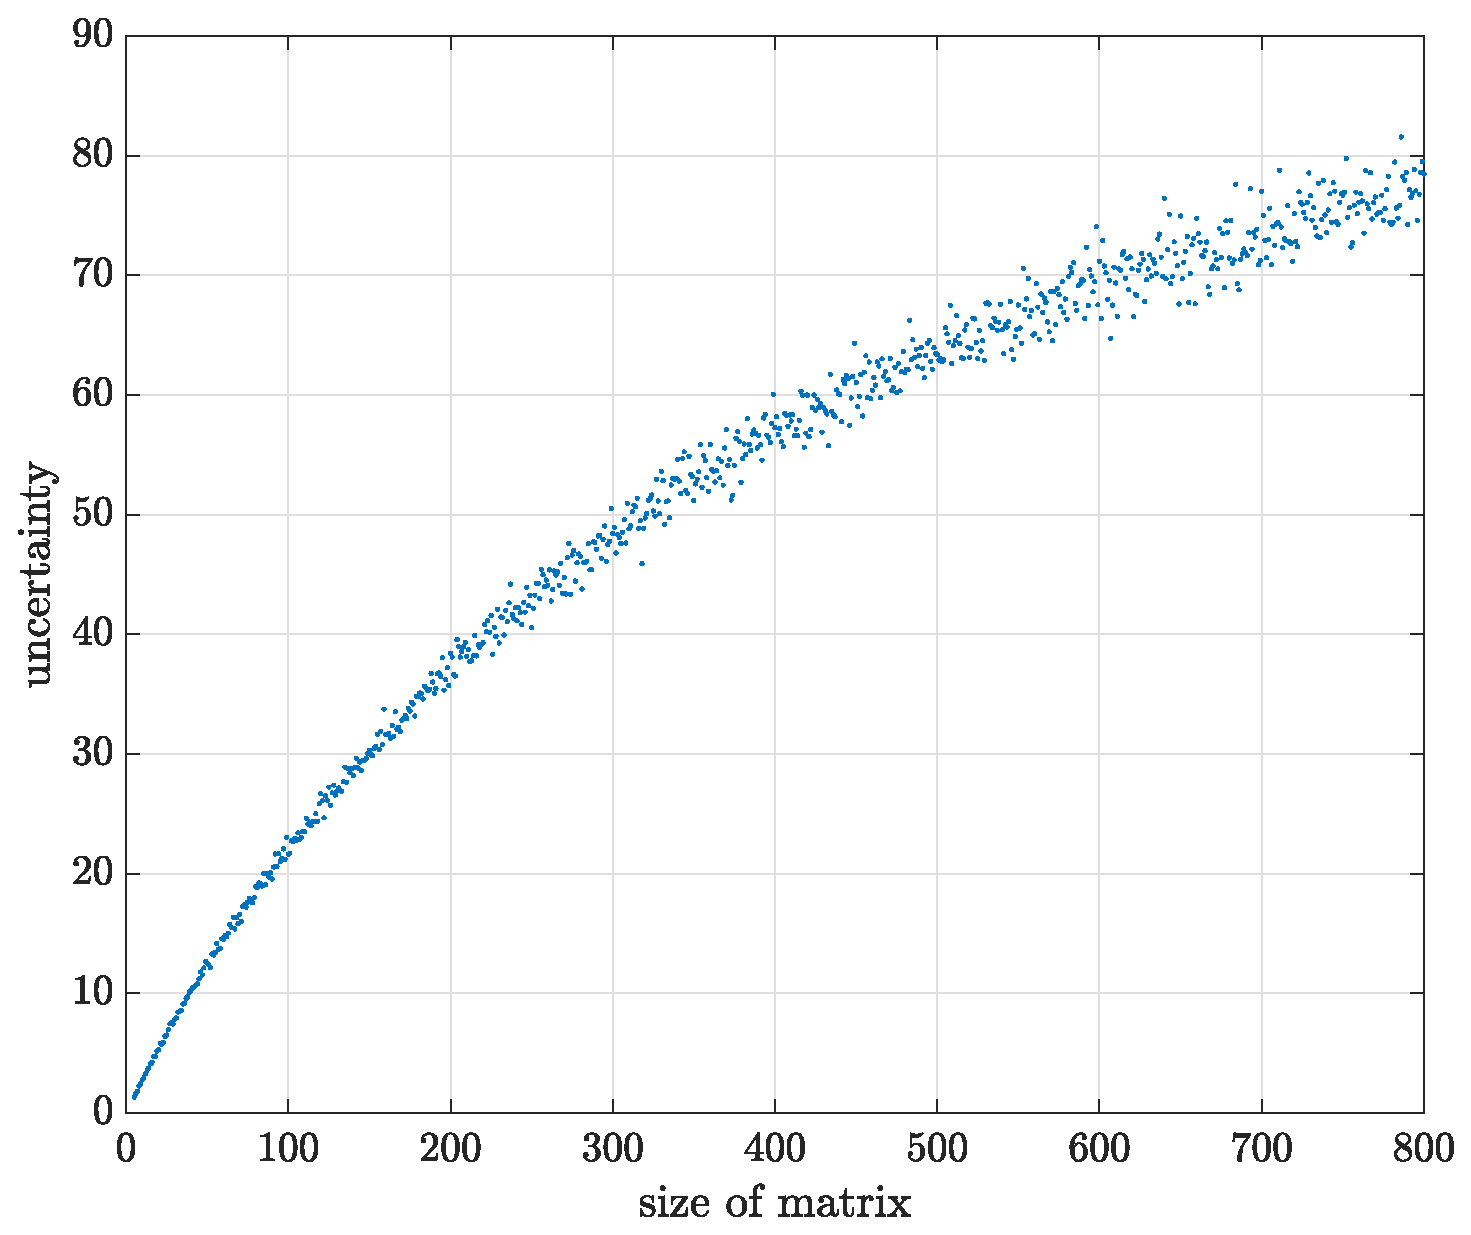
\includegraphics[scale=0.3]{figs/uncertainty_size_c}
            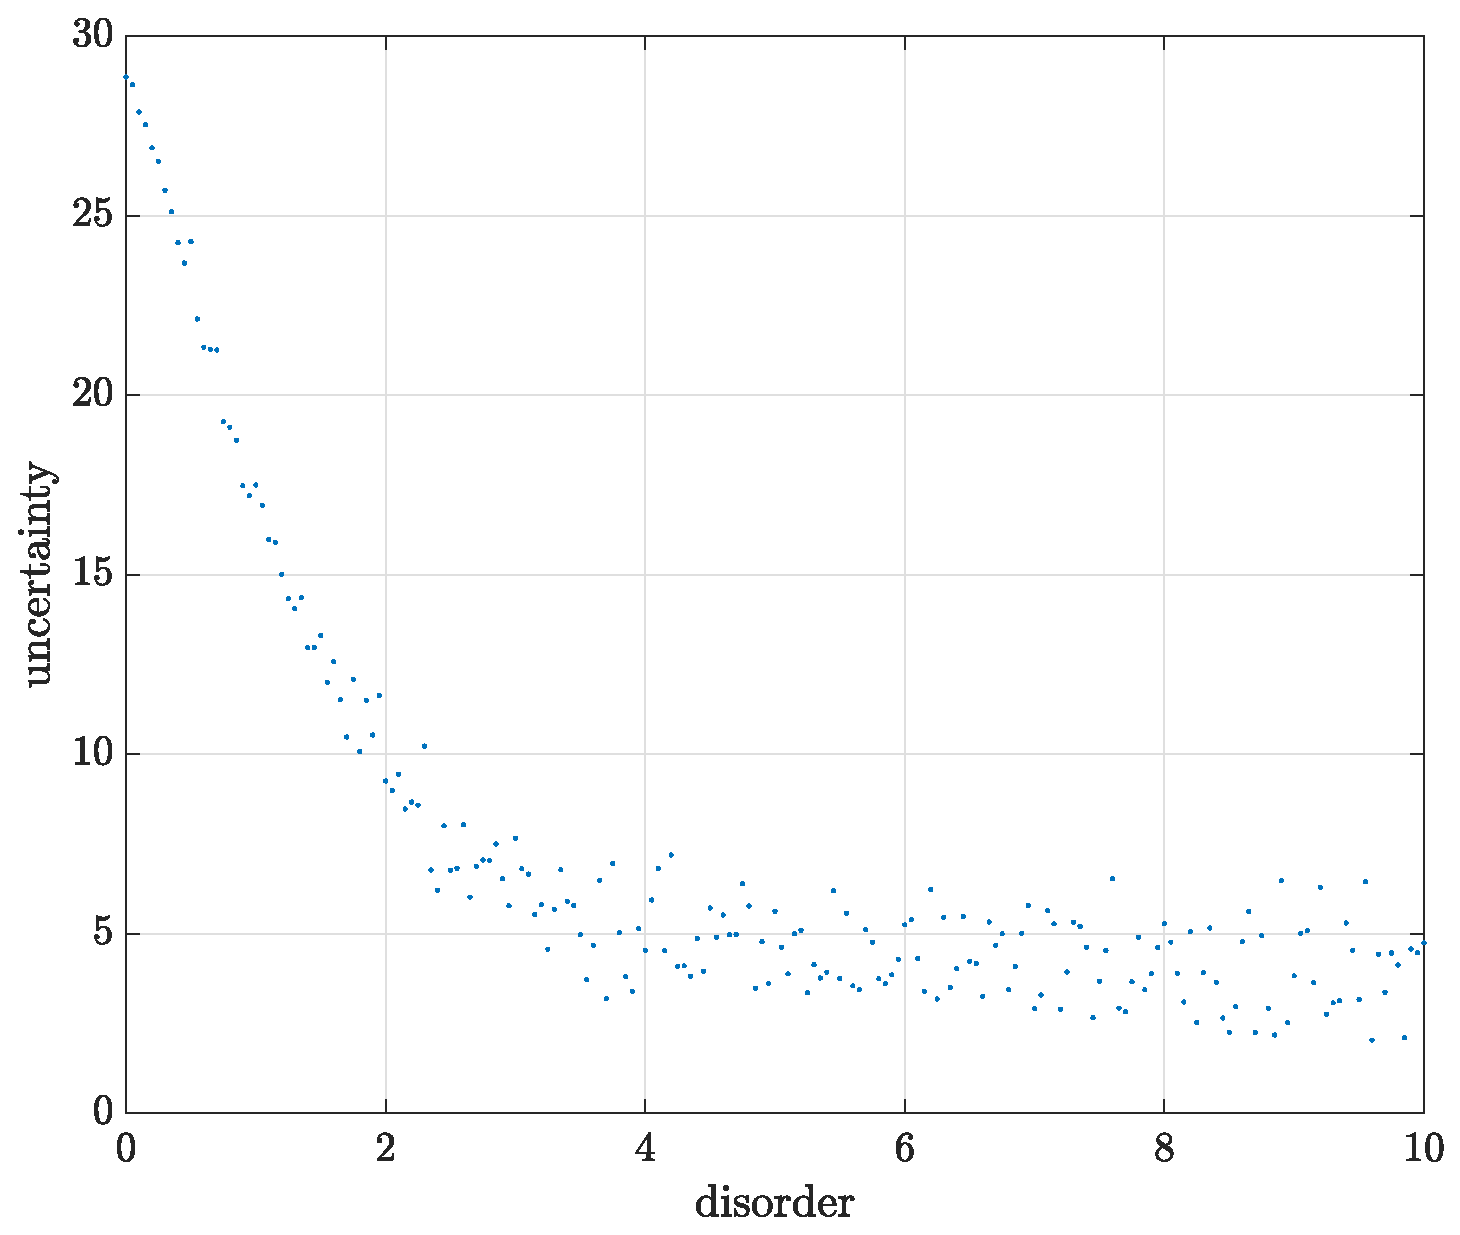
\includegraphics[scale=0.3]{figs/uncertainty_disorder_c}
            \caption{Uncertainty depending on size or disorder}
            \label{uncertainty_fig}
        \end{figure}
\end{homeworkProblem}

\begin{homeworkProblem}
    \begin{homeworkSection}{(1) classic Jacobi method}
        \matlabscript{MatLab/eig_j}{A Matlab script that compute the classic Jacobi method}
    \end{homeworkSection}
    \begin{homeworkSection}{(2) cyclic Jacobi method}
        \matlabscript{MatLab/eig_cj}{A Matlab script that compute the cyclic Jacobi method}
        
        Figures~\ref{figs/Jacobi_rotation_size_c} and~\ref{figs/Jacobi_Time_size_c} show the difference of calculation between classic (j) and cyclic (cj) Jacobi methods. As one can see, cyclic methods is way faster, even through it's required more rotations. This can be explained by the fact that searching the maximum is in O(N$^2$) and a rotation (without using Matrix multiplication is in O(N).
        
        \scalefig{figs/Jacobi_rotation_size_c}{0.65}{Comparison average number of rotations required for the diagonalisation of random matrix between classic and cyclic Jacobi methods}
        \scalefig{figs/Jacobi_Time_size_c}{0.65}{Comparison average time required for the diagonalisation of random matrix between classic and cyclic Jacobi methods}
    \end{homeworkSection}
\end{homeworkProblem}

\begin{homeworkProblem}
    \begin{homeworkSection}{(1) matrix representations}
        Table~\ref{tab_matrix_size} shows how much Bytes in memory are necessary to store an N$^2\times$N$^2$ Hamiltonian matrix. Sparse matrix clearly use less Bytes, and allow us to store bigger matrix. The figure~\ref{figs/matrix_time_c} shows an other interesting thing about sparse matrix; they are way faster to compute as N increase.
        \begin{table}[h]
            \centering
            \begin{tabular}{|c|c|c|}
                \hline
                N & full matrix [Bytes] & sparse matrix [Bytes]  \\
                \hline
                \hline
                30 & 6'480'000 & 77'288 \\
                100 & 800'000'000 & 873'608 \\
                1000 & 7'450.6$\cdot 10^9$ (Estimated) & 87'936'008 \\
                \hline
            \end{tabular}
            \caption{Memory size required to store the Hamiltonian matrix depending on N for full and sparse matrix}
            \label{tab_matrix_size}
        \end{table}
        \scalefig{figs/matrix_time_c}{0.6}{Time needed to create an N$^2\times$N$^2$ Hamiltonian matrix for full and sparse matrix}
    \end{homeworkSection}
    
    \begin{homeworkSection}{(2) bound solutions}
        Searching for the number of bound solutions using the Hamiltonian calculated above gives us, for N$= 100, r = 5\nano\meter$ and $a=5r$, the result that there are 90 bound solutions. The three lowest are given in table~\ref{tab_probability_Ei} along with their energy and their probability to find the particle inside the quantum well. One can see that the second one is two times degenerated. The three figure~\ref{E1_fig},~\ref{E2_fig} and~\ref{E3_fig} show their wave function and probability density. As one can see, the probability obtained in table~\ref{tab_probability_Ei} can be verified on this figure.
        
        \begin{table}[h]
            \centering
            \begin{tabular}{|c|c|c|}
                \hline
                $E_i$ & Energy [eV] & Probability \\
                \hline
                \hline
                $E_1$ & -0.4921 & 99.92 \% \\
                $E_2$ & -0.4799 & 99.80 \% \\
                $E_3$ & -0.4799 & 99.80 \% \\
                \hline
            \end{tabular}
            \caption{Energy and probability to find the particle inside the quantum well for the three lowest energy}
            \label{tab_probability_Ei}
        \end{table}
        
        \begin{figure}[H]
            \centering
            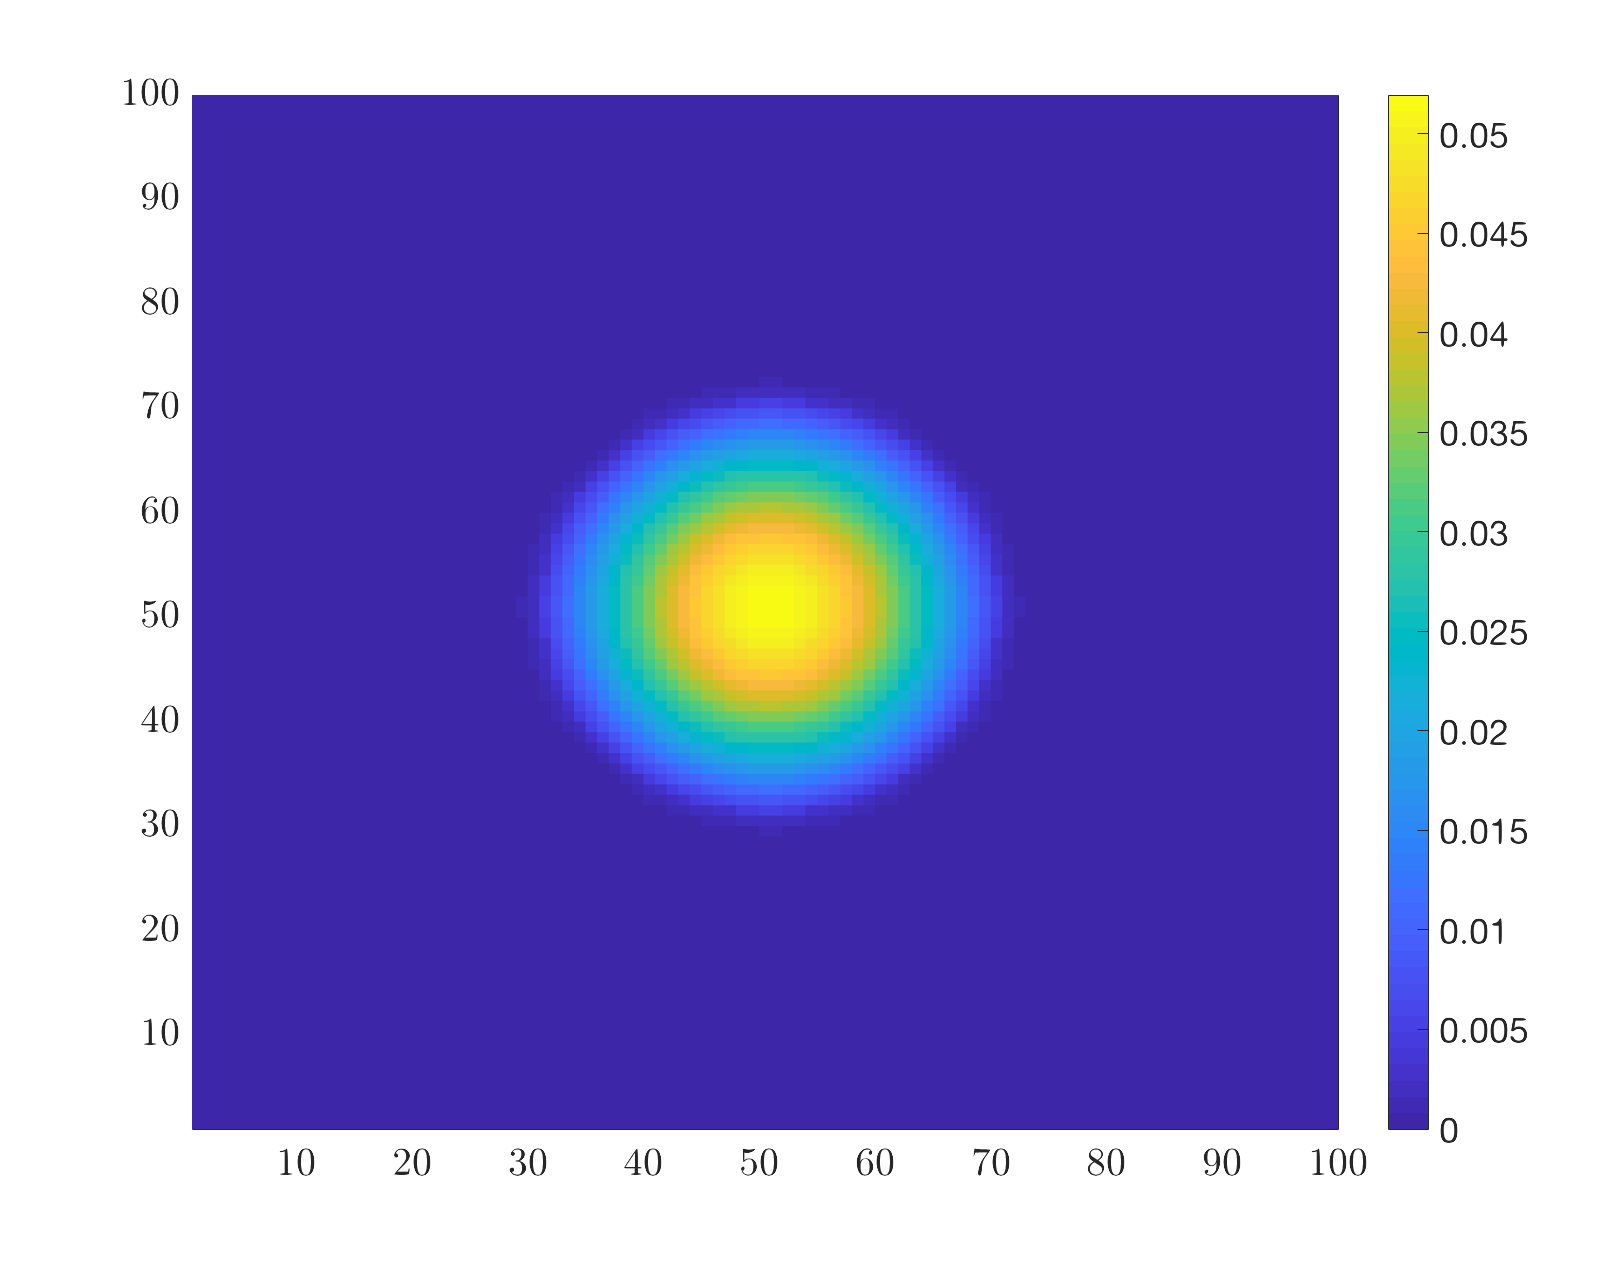
\includegraphics[scale=0.13]{figs/E1_wavefunction}
            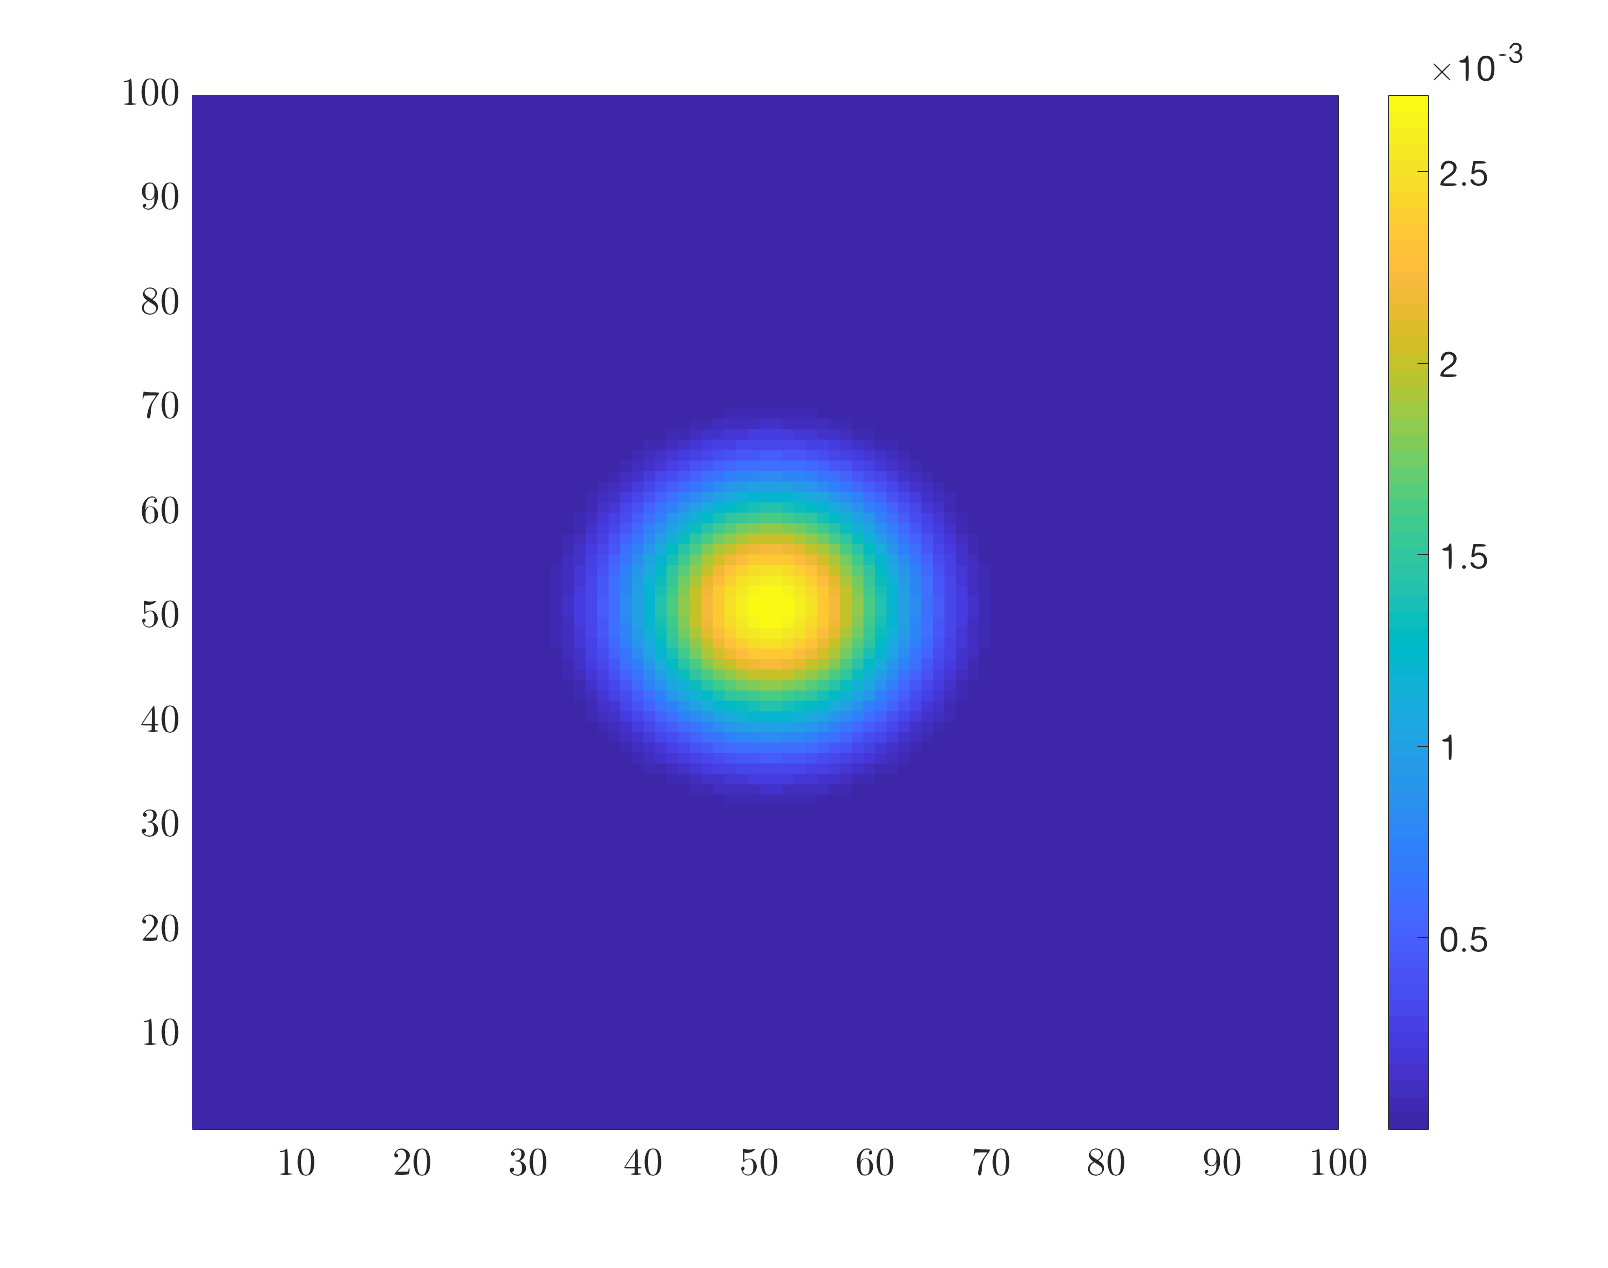
\includegraphics[scale=0.13]{figs/E1_probability_density}
            \caption{$E_1$ wave function and probability density}
            \label{E1_fig}
        \end{figure}
        \begin{figure}[H]
            \centering
            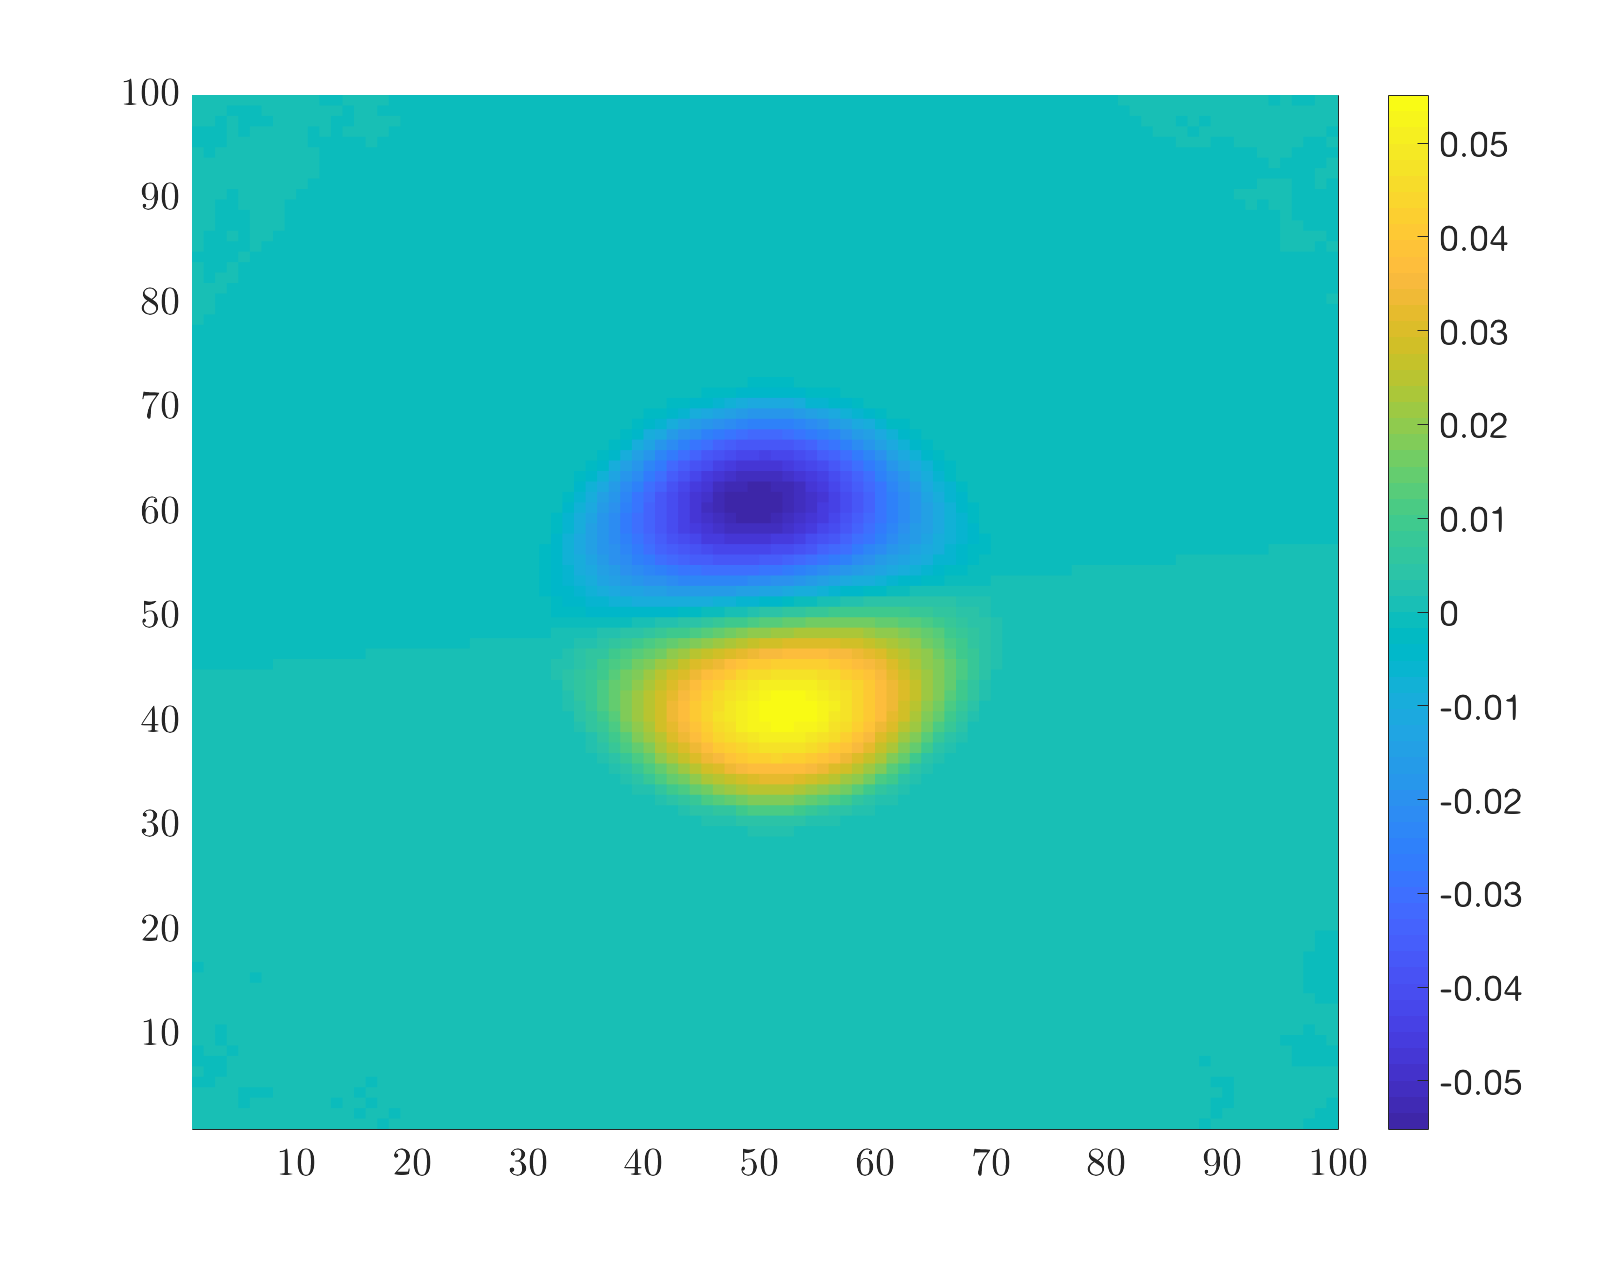
\includegraphics[scale=0.13]{figs/E2_wavefunction}
            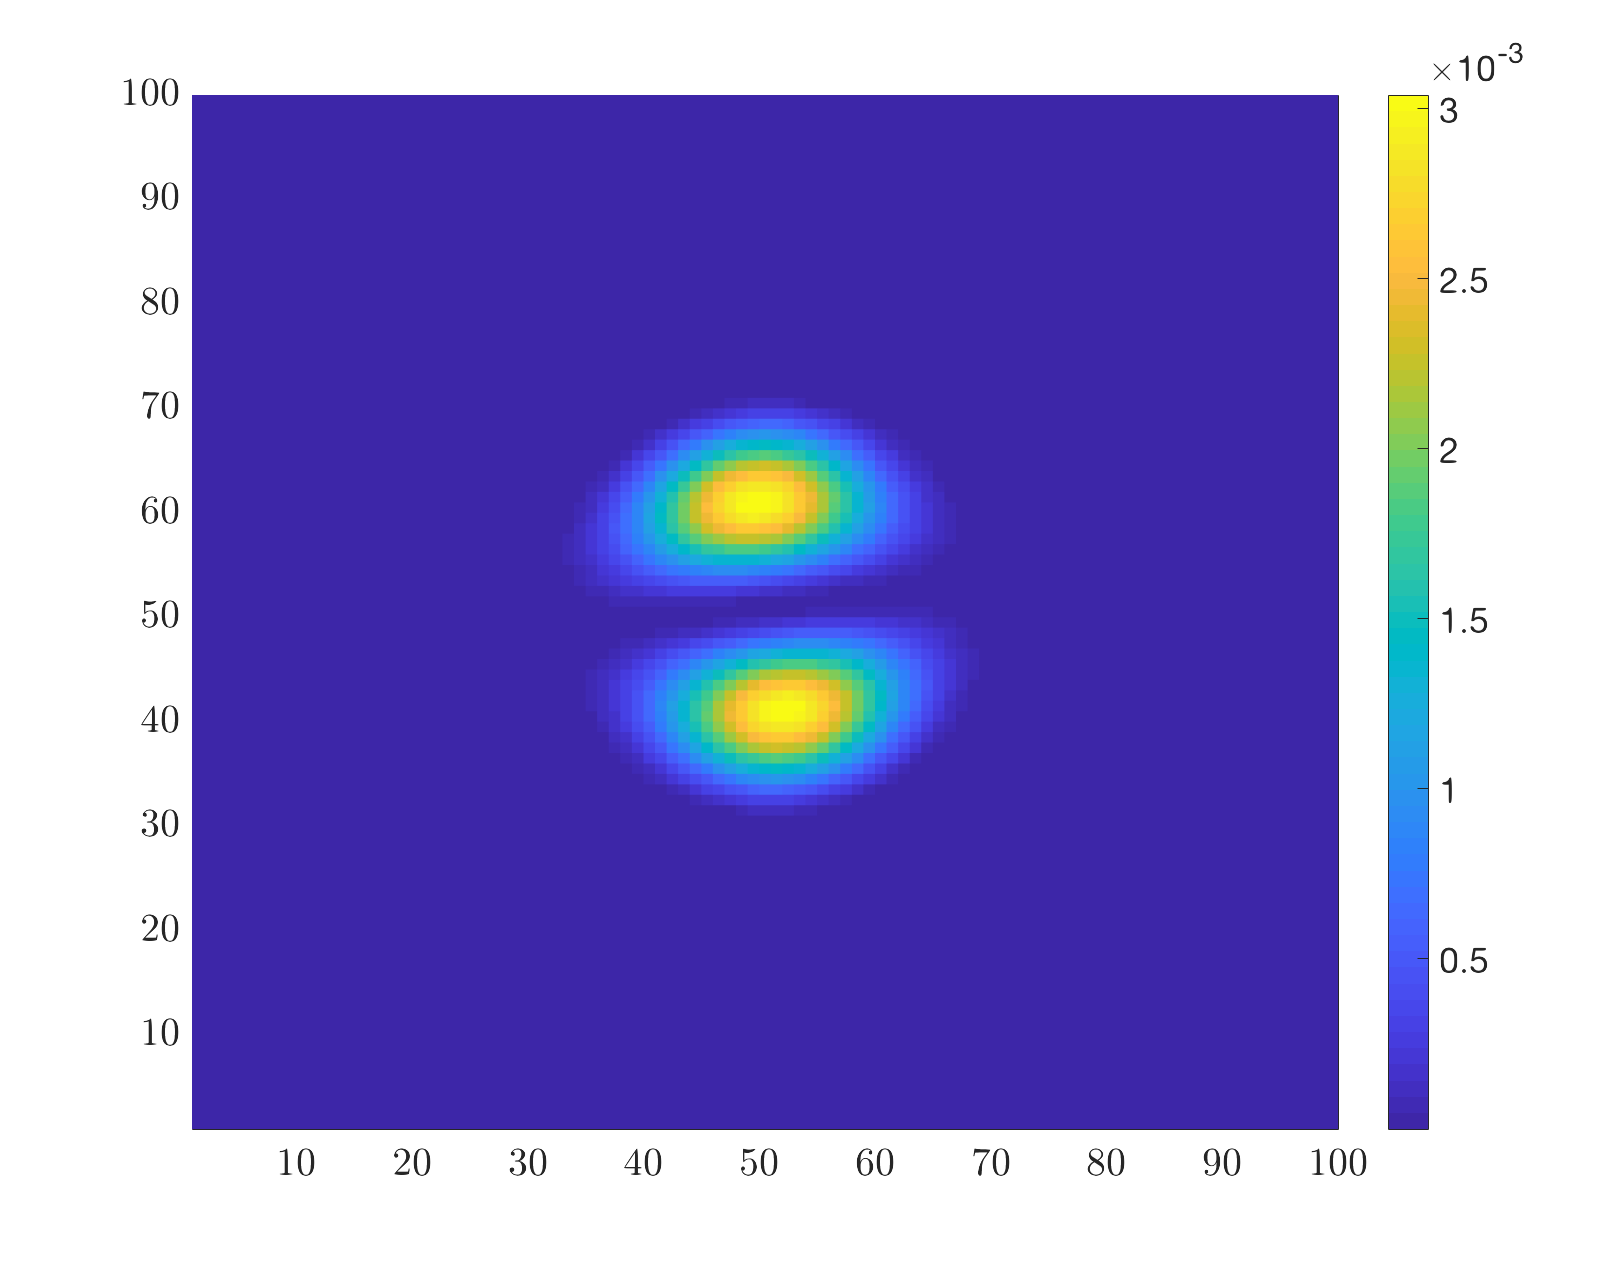
\includegraphics[scale=0.13]{figs/E2_probability_density}
            \caption{$E_2$ wave function and probability density}
            \label{E2_fig}
        \end{figure}
        \begin{figure}[H]
            \centering
            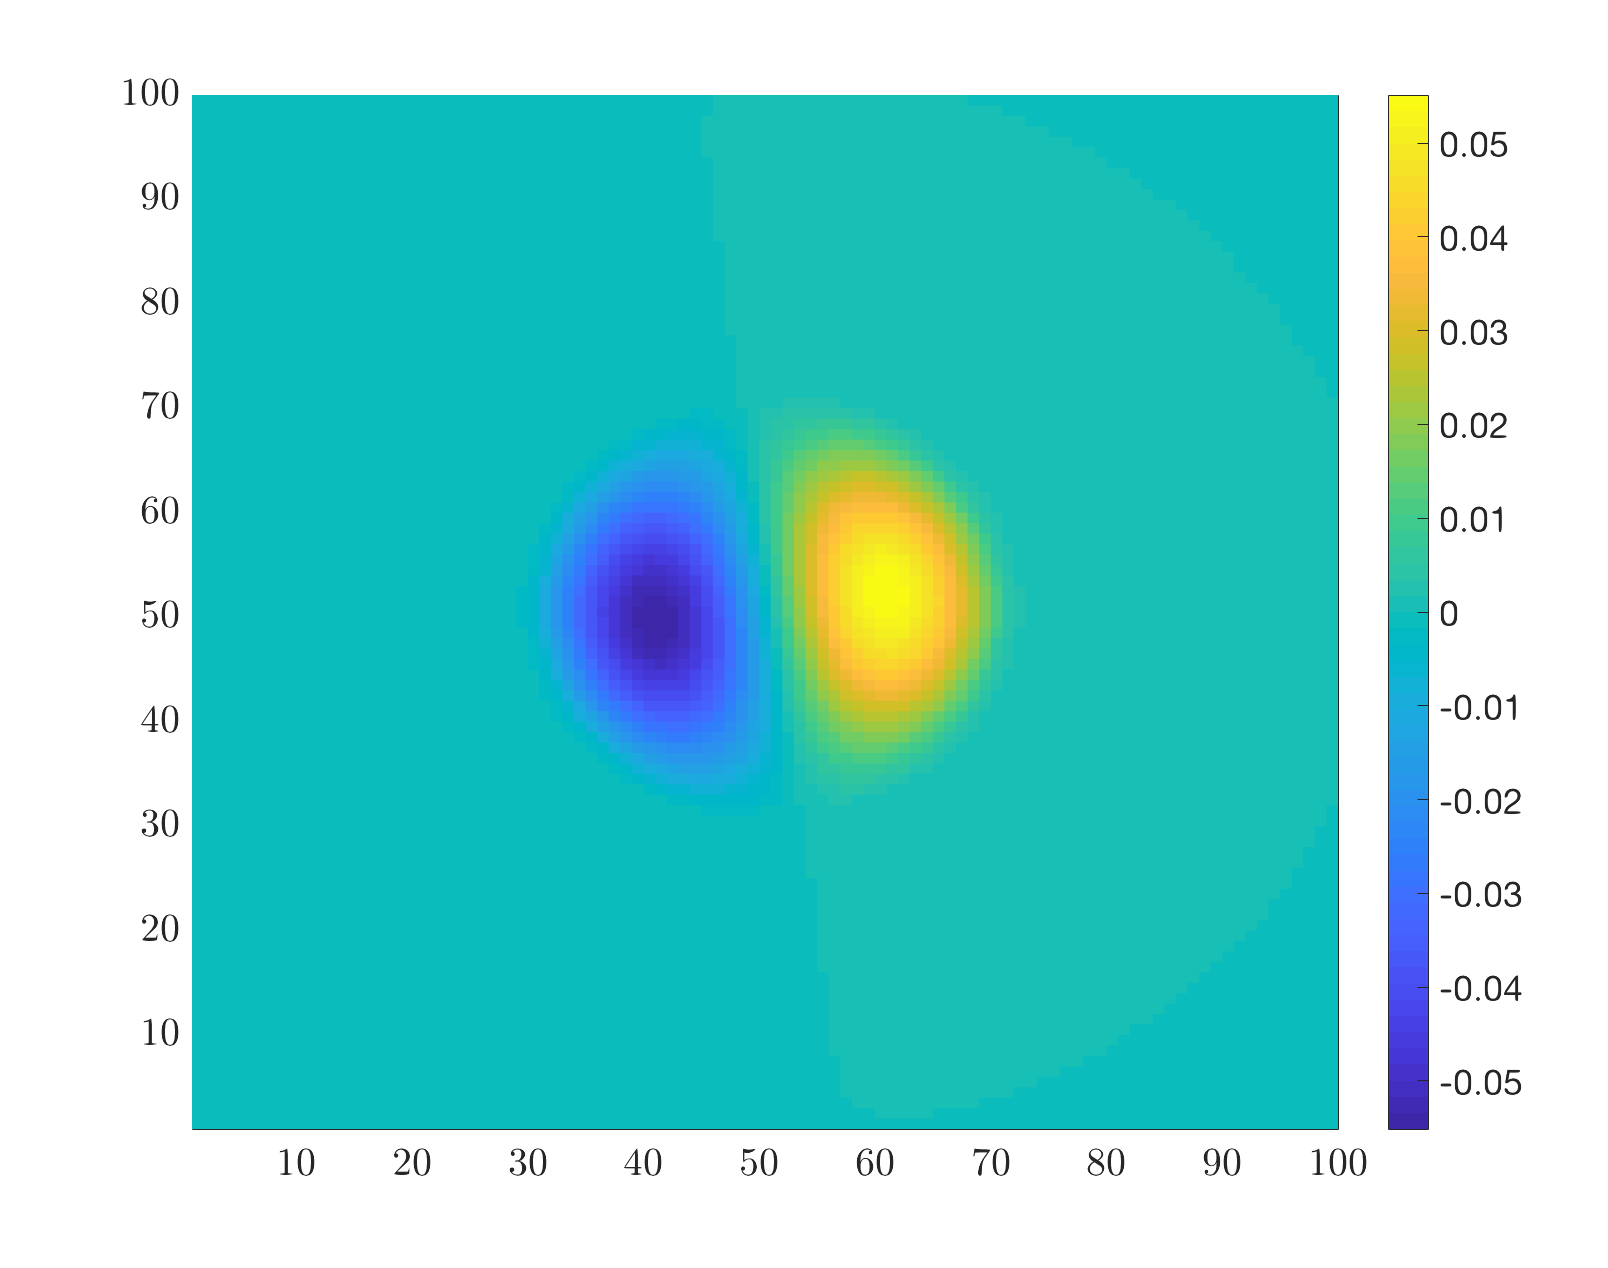
\includegraphics[scale=0.13]{figs/E3_wavefunction}
            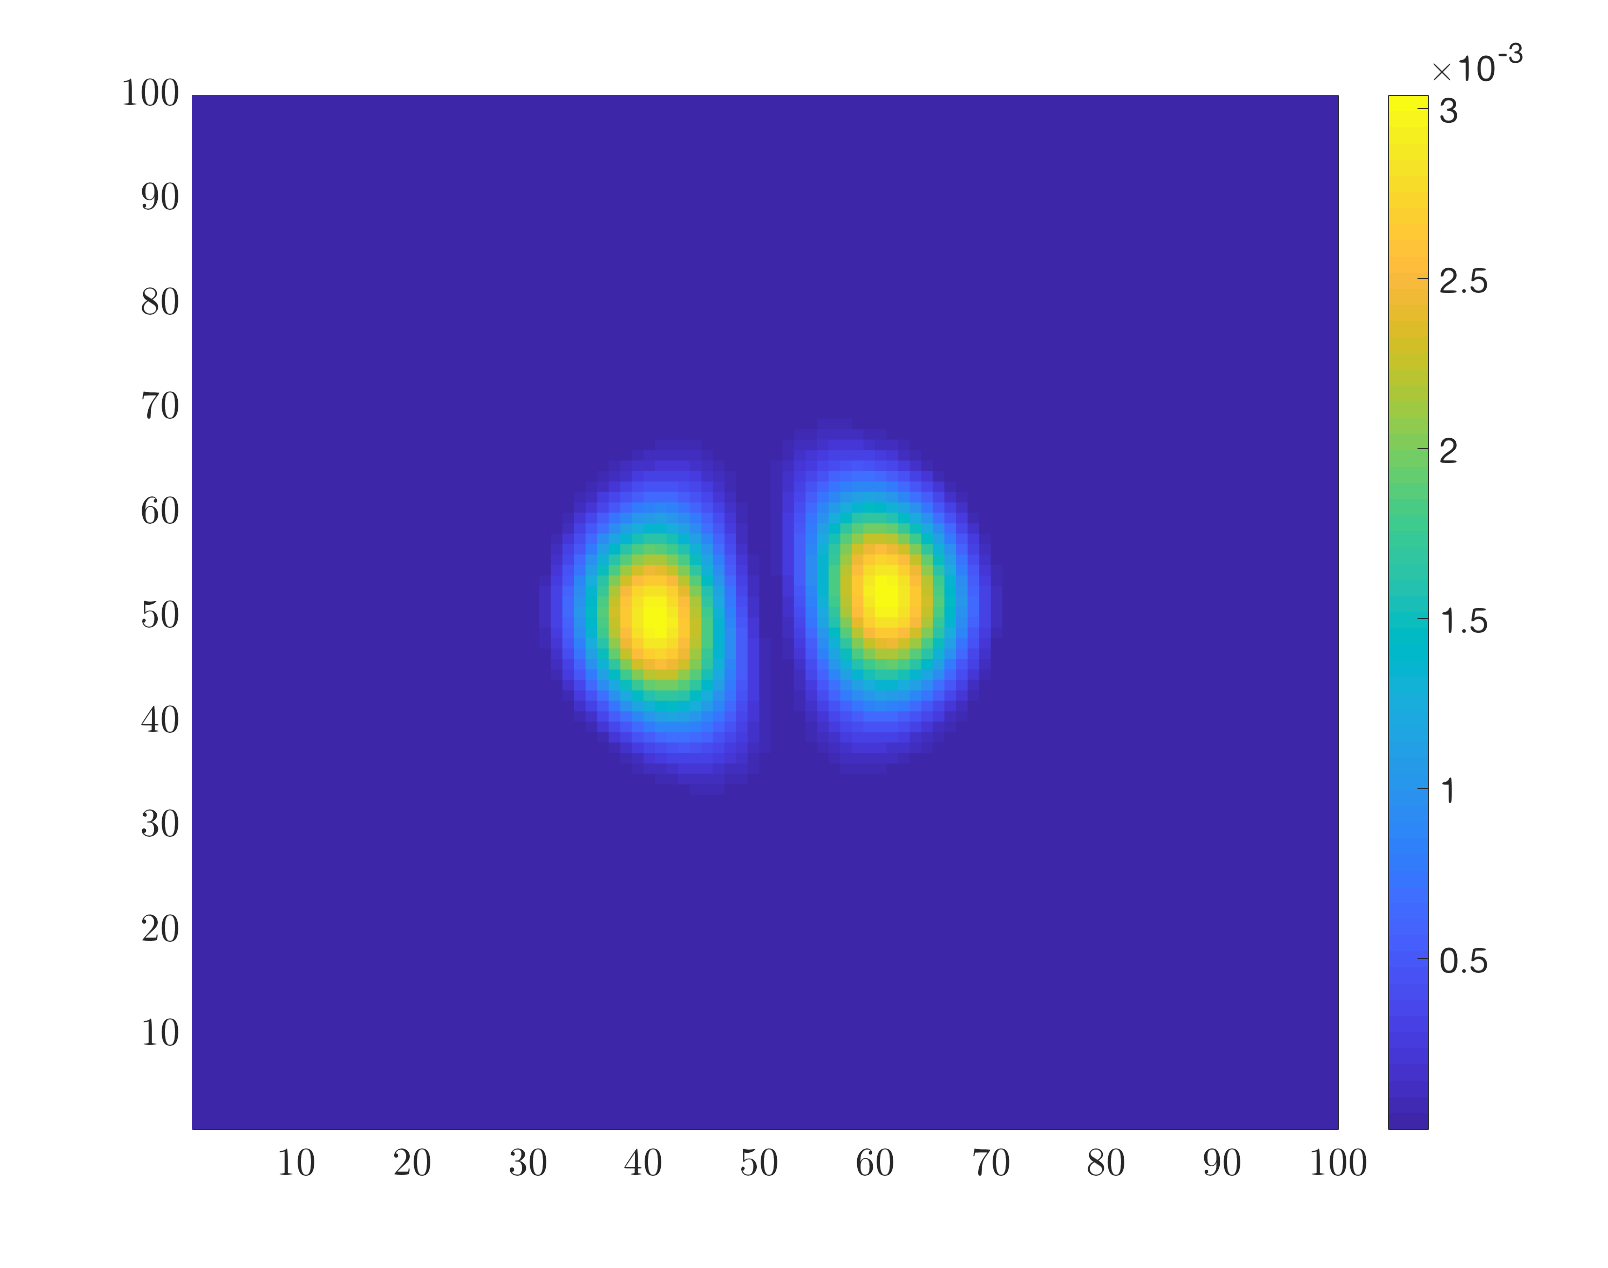
\includegraphics[scale=0.13]{figs/E3_probability_density}
            \caption{$E_3$ wave function and probability density}
            \label{E3_fig}
        \end{figure}
    \end{homeworkSection}
    
    \begin{homeworkSection}{(3) scattering solutions}
        The figure~\ref{Eapprox1_fig} show the wave function and the probability density for energy close to 1. As one can see, the probability to find the particle inside the quantum well is very different than the one for $E_1, E_2$ or $E_3$. In fact, this probability is now $12.02\%$. The figure~\ref{figs/Eapprox1_probability_c} shows the decency of this probability in term of $a$.
        
        \begin{figure}[H]
            \centering
            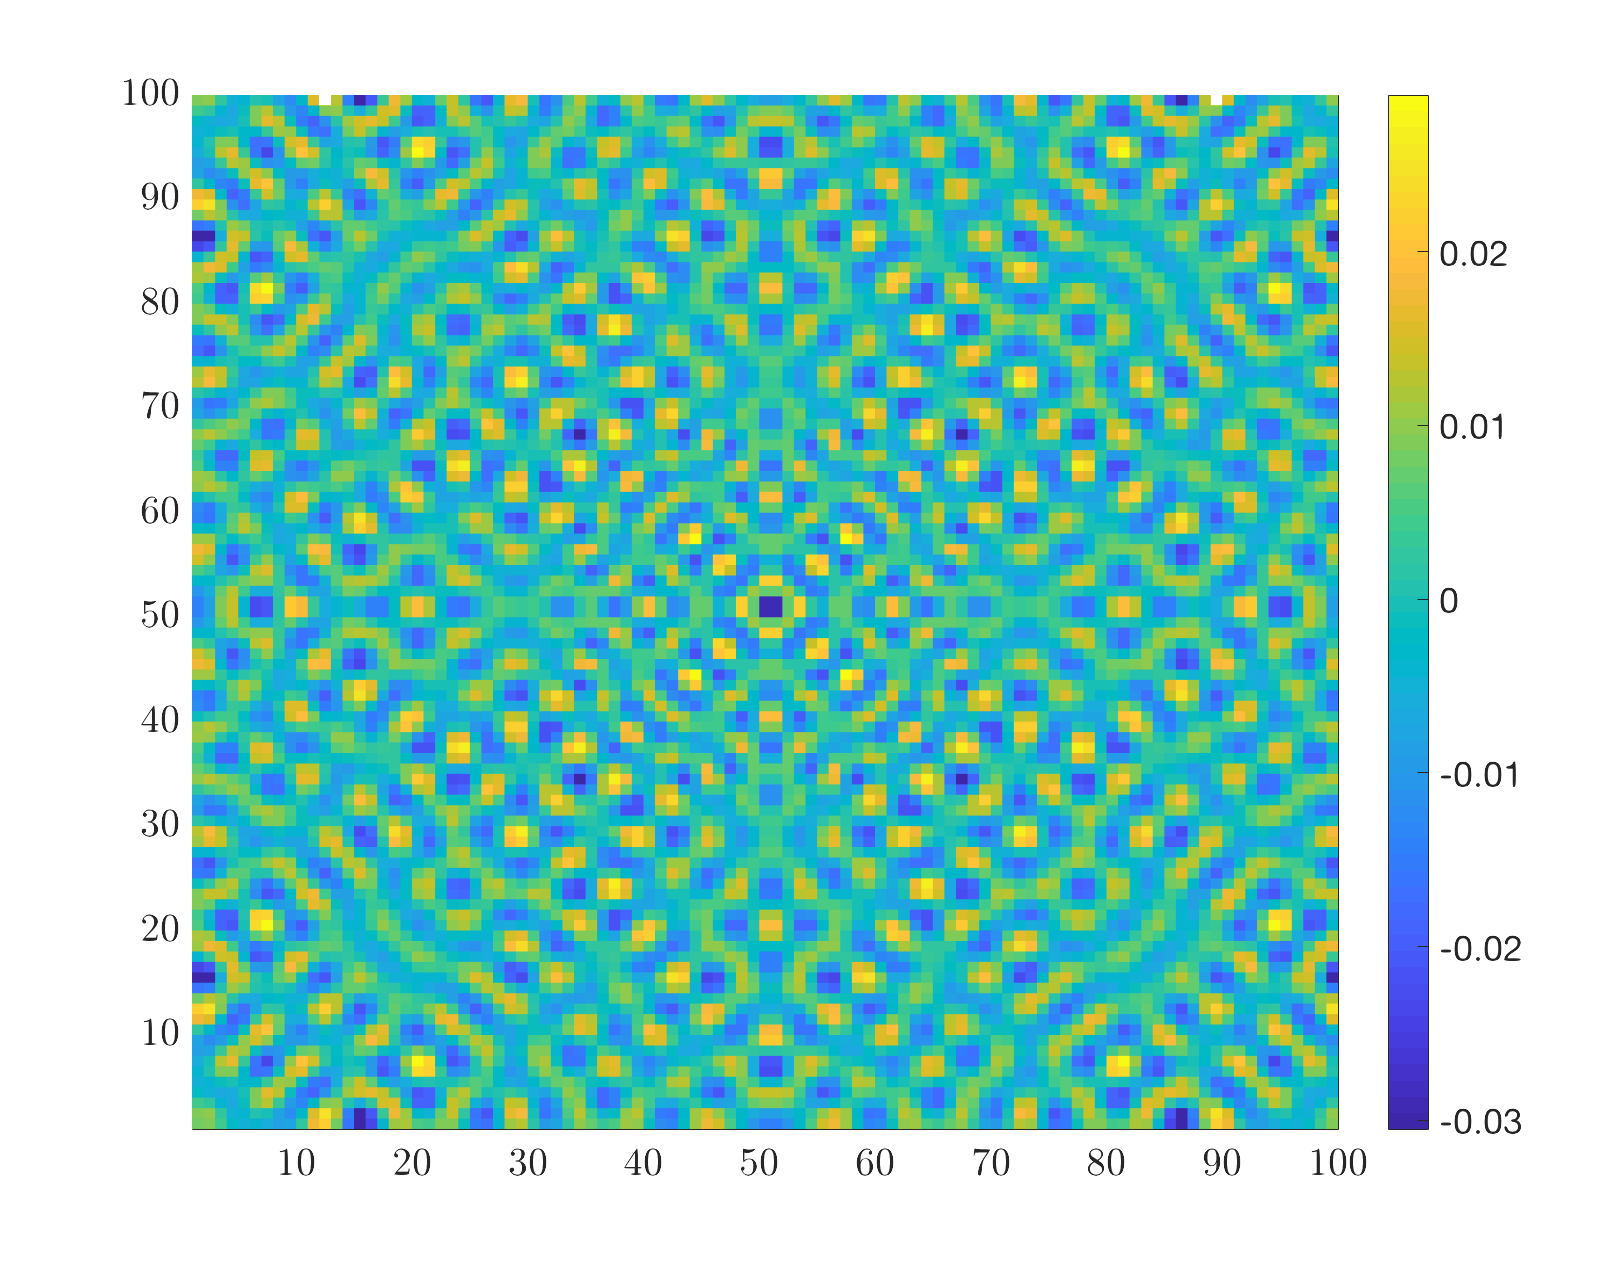
\includegraphics[scale=0.13]{figs/Eapprox1_wavefunction}
            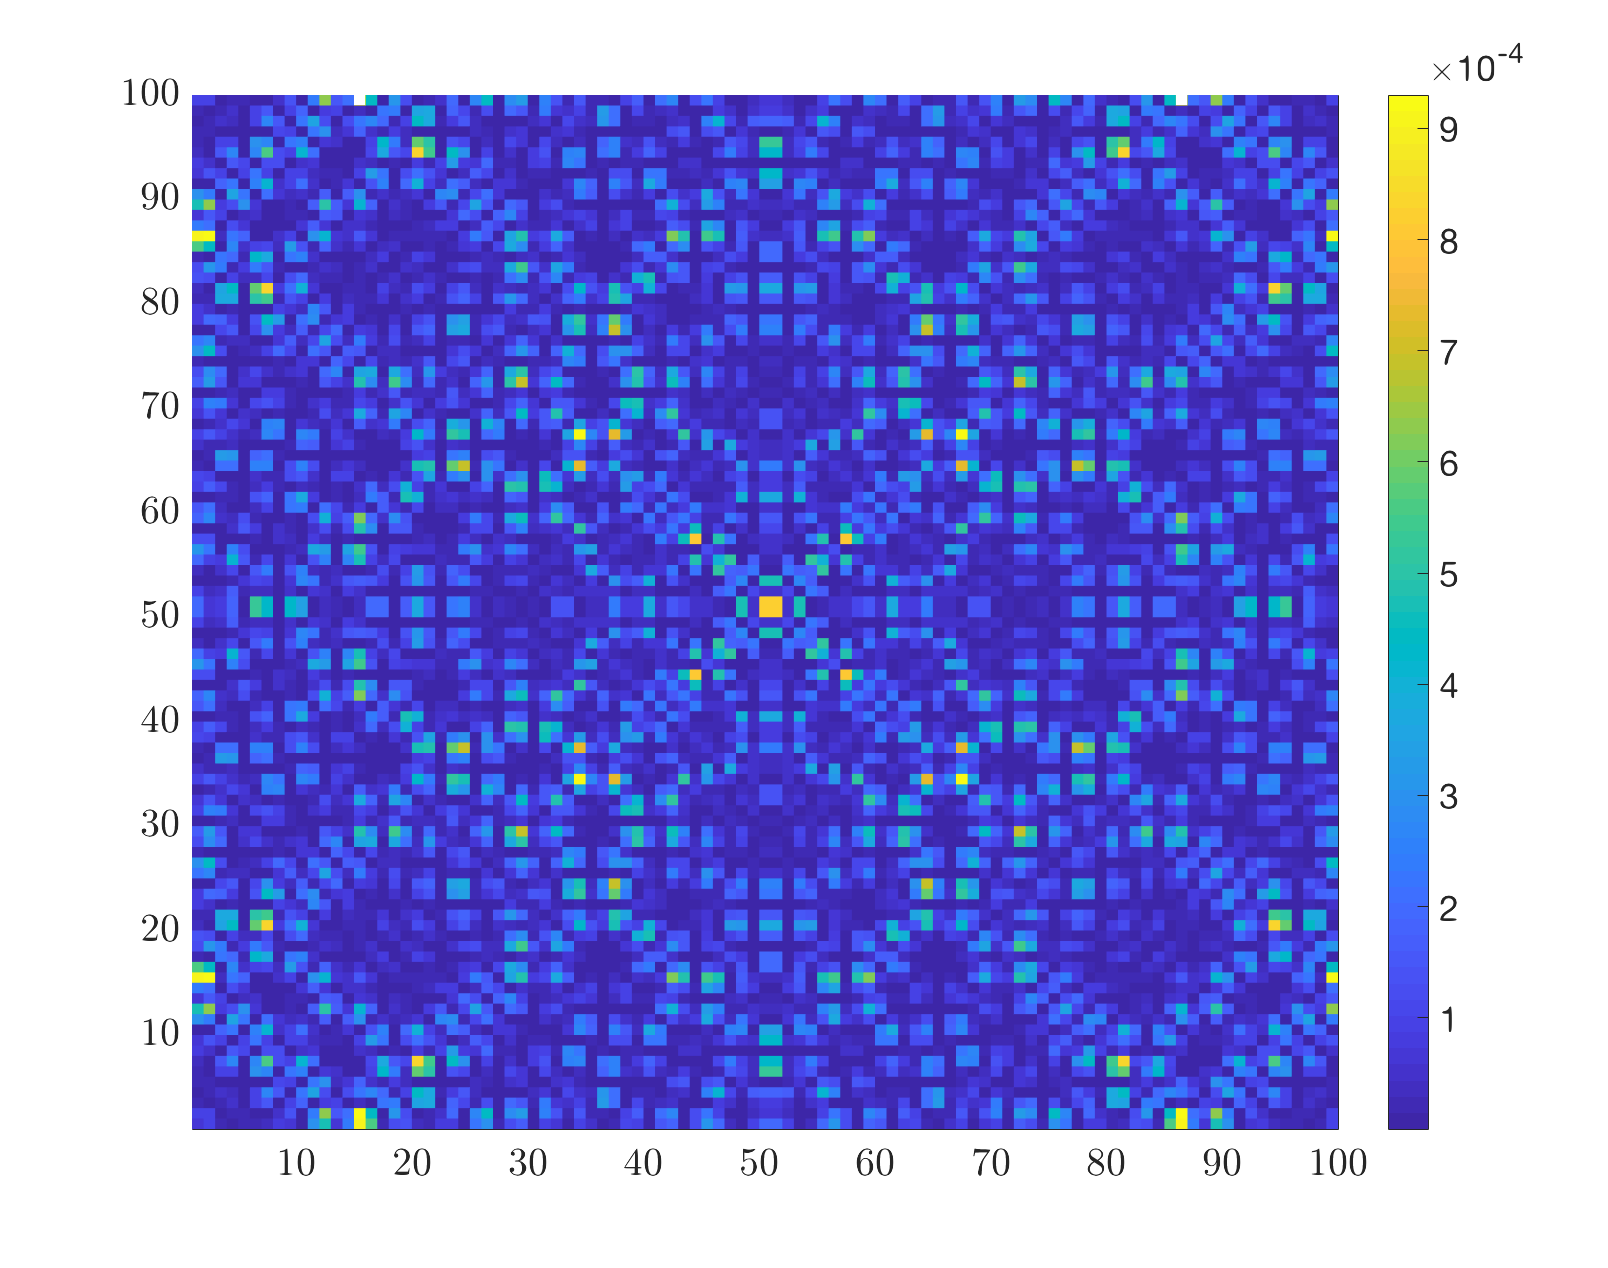
\includegraphics[scale=0.13]{figs/Eapprox1_probability_density}
            \caption{$E \approx 1$ wave function and probability density}
            \label{Eapprox1_fig}
        \end{figure}
        \scalefig{figs/Eapprox1_probability_c}{0.6}{Probability to find the particle inside the quantum well depending on $a$}
    \end{homeworkSection}
\end{homeworkProblem}

\newpage

%			Bibliographie
\begin{thebibliography}{99}

\bibitem{notice_gen}

\textit{Exercise sessions 6–7: LU decomposition and systems of linear equations.} written by O. Yazyev, D. Pasquier, M. Pizzochero, R. Fournier in 2017-2018

\bibitem{laBible}

\textit{Exercise sessions 8-9: Diagonalization algorithms and eigenvalue problems} written by O. Yazyev, D. Pasquier, M. Pizzochero, R. Fournier in 2017-2018



\end{thebibliography}

\end{spacing}
\end{document}

%%%%%%%%%%%%%%%%%%%%%%%%%%%%%%%%%%%%%%%%%%%%%%%%%%%%%%%%%%%%%

